
\documentclass[runningheads,a4paper,11pt]{report}

\usepackage{algorithmic}
\usepackage{algorithm} 
\usepackage{array}
\usepackage{amsmath}
\usepackage{amsfonts}
\usepackage{amssymb}
\usepackage{amsthm}
\usepackage{caption}
\usepackage{comment} 
\usepackage{epsfig} 
\usepackage[T1]{fontenc}
\usepackage{geometry} 
\usepackage{graphicx}
\usepackage[driverfallback=dvipdfm,colorlinks]{hyperref} 
\usepackage[latin1]{inputenc}
\usepackage{multicol}
\usepackage{multirow} 
\usepackage{rotating}
\usepackage{setspace}
\usepackage{subfigure}
\usepackage{url}
\usepackage{verbatim}
\usepackage{indentfirst}
\geometry{a4paper,top=3cm,left=2cm,right=2cm,bottom=3cm}


\newcolumntype{L}[1]{>{\raggedright\let\newline\\\arraybackslash\hspace{0pt}}m{#1}}
\newcolumntype{C}[1]{>{\centering\let\newline\\\arraybackslash\hspace{0pt}}m{#1}}
\newcolumntype{R}[1]{>{\raggedleft\let\newline\\\arraybackslash\hspace{0pt}}m{#1}}


\hypersetup{
pdftitle={artTitle},
pdfauthor={name},
pdfkeywords={pdf, latex, tex, ps2pdf, dvipdfm, pdflatex},
bookmarksnumbered,
pdfstartview={FitH},
urlcolor=cyan,
colorlinks=true,
linkcolor=red,
citecolor=green,
}
\pagestyle{plain}

\setcounter{secnumdepth}{3}
\setcounter{tocdepth}{3}

\linespread{1}

\pagestyle{myheadings}

\makeindex


\begin{document}

\begin{titlepage}
\sloppy
\begin{center}
BABE\c S BOLYAI UNIVERSITY, CLUJ NAPOCA, ROM\^ ANIA

FACULTY OF MATHEMATICS AND COMPUTER SCIENCE

SPECIALIZATION SOFTWARE ENGINEERING 

\vspace{5cm}

\Huge \textbf{Tracking progress of rehabilitation therapy using AI}

\vspace{1cm}

\normalsize -- Research Project --

\end{center}


\vspace{5cm}

\begin{flushleft}
\textbf{Supervisor} \break
\Large{\textbf{Lect. Dr. Ioan Lazar}}
\end{flushleft}

\begin{flushright}
\textbf{Author} \break
\Large{\textbf{Razvan Timis}}
\end{flushright}

\vspace{4cm}

\begin{center}
2019
\end{center}

\end{titlepage}

\pagenumbering{gobble}

\renewcommand{\contentsname}{Table of Contents}
\tableofcontents

% \newpage

% \listoftables
% \listoffigures
% \listofalgorithms

\newpage

\setstretch{1.5}

\begin{abstract}
\par In Physiotherapy, tracking Range of Motion (ROM) is a standard approach to measuring progress in patient therapy. Often, ROM is measured subjectively and documentation is inconsistent between clinicians.
\par Physios might come to wrong conclusions if ROM is tracked incorrectly between therapy sessions.
\par The problem is that up to 70\% of patients give up physiotherapy because they can not see immediate results.
\par That\mbox{'}s why we want to make a mobile application which makes use of a phone camera to objectively calculate ROM in real-time and automatically produce a report that tracks progress over the course of several therapy sessions.
In Physiotherapy, tracking Range of Motion (ROM) is a standard approach to measuring progress in patient therapy. Often, ROM is measured subjectively and documentation is inconsistent between clinicians. Physios might come to wrong conclusions if ROM is tracked incorrectly between therapy sessions.
The problem is that up to 70\% of patients give up physiotherapy because they can not see immediate results.\break
That\mbox{'}s why we want to make a mobile application which makes use of a phone camera to objectively calculate ROM in real-time and automatically produce a report that tracks progress over the course of several therapy sessions.
In Physiotherapy, tracking Range of Motion (ROM) is a standard approach to measuring progress in patient therapy. Often, ROM is measured subjectively and documentation is inconsistent between clinicians. Physios might come to wrong conclusions if ROM is tracked incorrectly between therapy sessions.
The problem is that up to 70\% of patients give up physiotherapy because they can not see immediate results.\break
That's why we want to make a mobile application which makes use of a phone camera to objectively calculate ROM in real-time and automatically produce a report that tracks progress over the course of several therapy sessions.

\end{abstract}

\newpage

\pagenumbering{arabic}

\chapter{Introduction}
\par In Physiotherapy, tracking Range of Motion (ROM) is a standard approach to measuring progress in patient therapy. Often, ROM is measured subjectively and documentation is inconsistent between clinicians. Physios might come to wrong conclusions if ROM is tracked incorrectly between therapy sessions.

\begin{figure}[htbp]
	\centerline{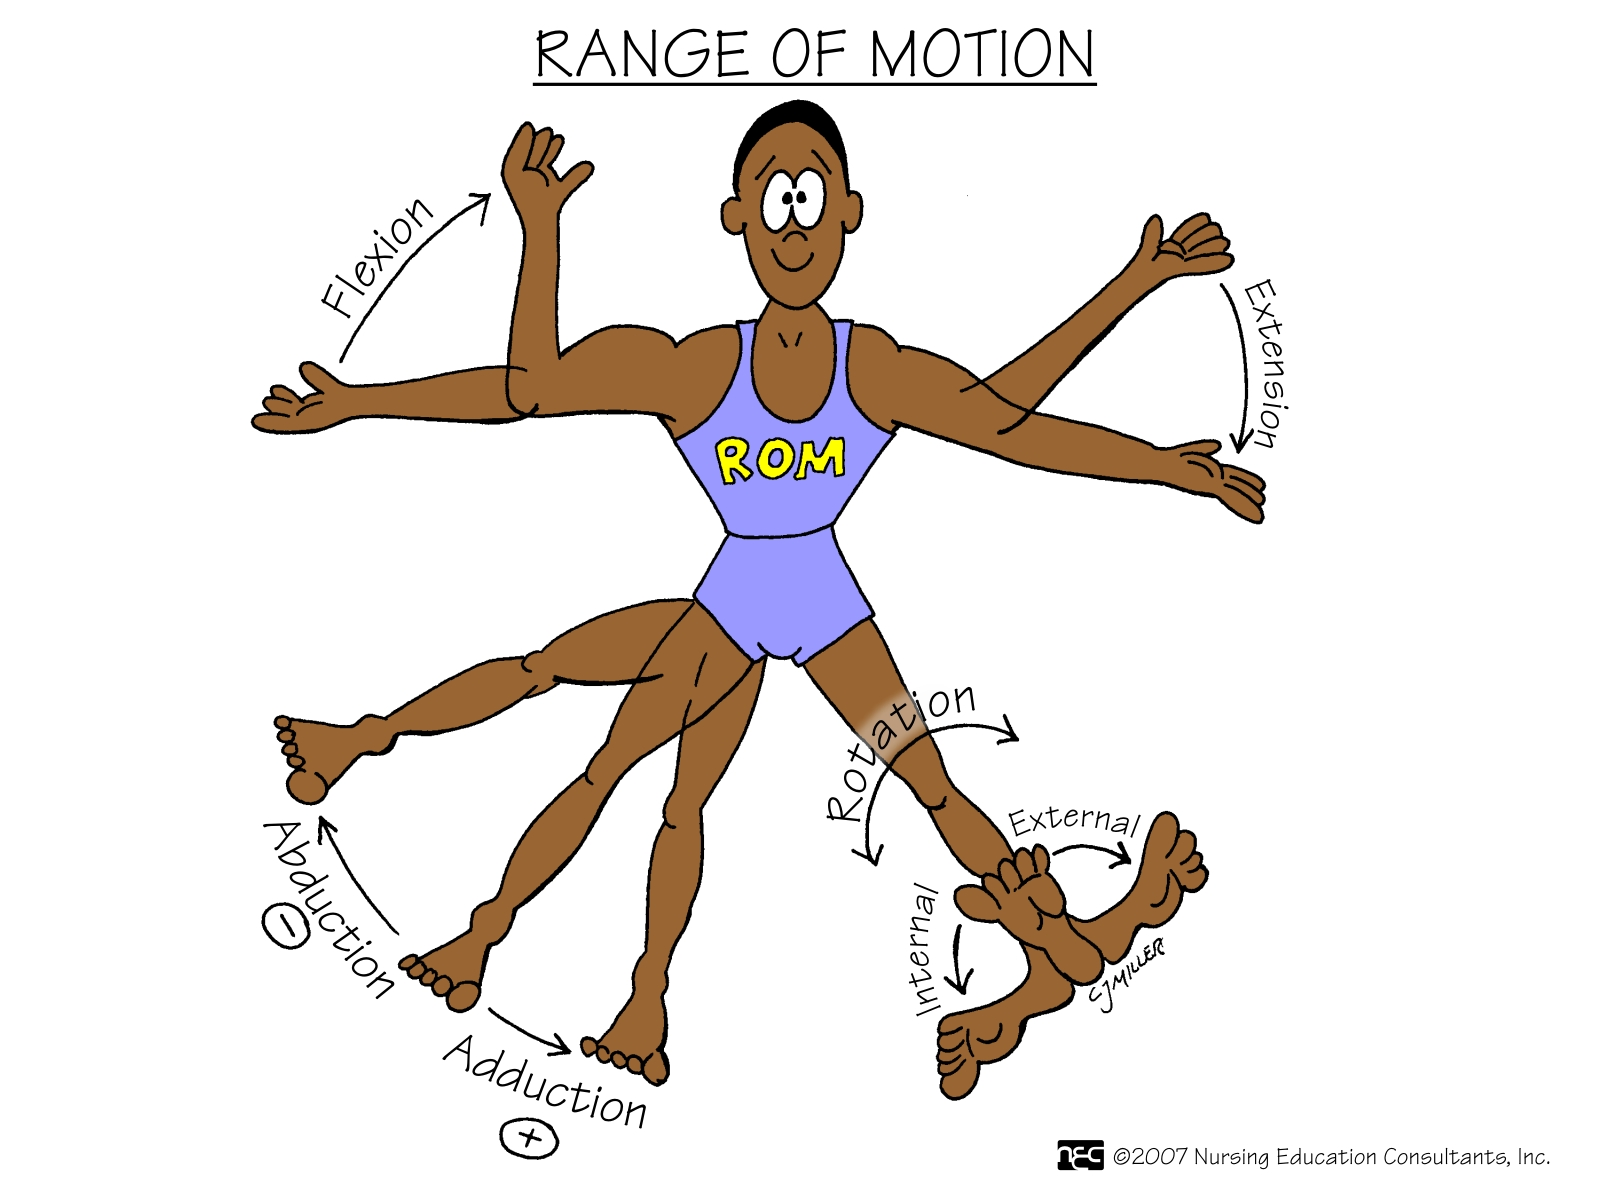
\includegraphics[scale=0.25]{fig/rangeofmotion.png}}  
	\caption{Range of Motion}
\end{figure}

\par The problem is that up to 70\% of patients give up physiotherapy because they can not see immediate results.
\par That's why we want to make a mobile application which makes use of a phone camera to objectively calculate ROM in real-time and automatically produce a report that tracks progress over the course of several therapy sessions.

\section{Motivation}
\par Our motivation is to help patients who need physiotherapy to see a progress and to encourage them to be constant during their treatment. We want to support patients motivation in continuing to build new and healthy behaviours. 
\par This application is designed to help everyone who need physiotherapy treatment to stay motivated, reach their goals, and create habits that are healthy and helpful for a long term. In this case we have a solution by creating a mobile app which will be a useful tool for patients who needs help to reach their goals by automated tracking of ROM.

\section{The purpose of the application}
\chapter{Related work}

\section{DeeperCut\mbox{:} A Deeper, Stronger, and Faster Multi-Person Pose Estimation Model \cite{DBLP:journals/corr/InsafutdinovPAA16}}

\subsection{Problem}
The goal of this paper is to advance the state-of-the-art of articulated pose estimation in scenes with multiple people.

\subsection{Methods}
\begin{itemize}
  \item improved body part detectors that generate effective bottom-up proposals for body parts.
  \item novel image-conditioned pairwise terms that allow to assemble the proposals into a variable number of consistent body part configurations.
  \item an incremental optimization strategy that explores the search space more efficiently thus leading both to better performance and significant speed-up factors.
\end{itemize}

\subsection{Data}
\begin{itemize}
    \item Datasets. Three public datasets are used: \mbox{"}Leeds Sports Poses\mbox{"} (LSP) (personcentric (PC) annotations)
    \item MPII Human Pose ( Single Person )  consisting of 19185 training and 7247 testing poses. To evaluate on LSP we train part detectors on the union of MPII, LSPET and LSP training sets. To evaluate on MPII Single Person we train on MPII only.
\end{itemize}
\subsection{Performance and comparisons}
Evaluation is done on two single-person and two multi-person pose estimation benchmarks. The proposed approach significantly outperforms best known multi-person pose estimation results while demonstrating competitive performance on the task of single person pose estimation.

\section{Human Pose Estimation from Monocular Images: A Comprehensive Survey
\cite{humanmonocular}}




\chapter{Application}
\chapter{Conclusion}
\par Proposed system for the tracking of the posture doesn\mbox{'}t perform as we originally expected.
\par There seems to be some problems regarding the determination of the bounding box, maybe due to the fact that the detected points are on a surface that is characterized by just a few colors that appear in almost all tracked region. Because of these characteristics of the tracked posture we fail to track enough points due to insufficient difference in the nearest proximity of a point. 

\par For future development we will try to adapt described system to track the contours.

Even if posture tracking system doesn\mbox{'}t perform as we expected, we succeeded in the finding the appropriate settings for the PoseNet so that it performs enough good for the determination of the ranges of motion. Based on these calculations we were able to count, in real time, the number of exercises that user made.


\bibliographystyle{plain}
\bibliography{BibAll}
\end{document}
